\documentclass[11pt,a4paper]{article}

\usepackage[T1]{fontenc}
\usepackage[utf8]{inputenc}
\usepackage{lmodern}
\usepackage[margin=2.5cm]{geometry}
\usepackage{graphicx}
\usepackage{booktabs}
\usepackage{amsmath}
\usepackage{caption}
\usepackage[section]{placeins}
\usepackage[numbers]{natbib}
\usepackage[hidelinks]{hyperref}

\graphicspath{{../figures/}{./}}
\captionsetup{font=small}

\title{Evaluating Lineage Link Prediction with Valentine\\[4pt]
\large Semantic Web -- Draft Report (Milestone 5)}
\author{Sema Sert, Yi\u{g}it Do\u{g}an, Alessandro Toro, Achraf Frigui\\[2pt]
\small Group 6 \quad\textbullet\quad \url{https://github.com/semasertt/valentine-lineage}}
\date{December 2026}

\begin{document}
\maketitle

\begin{abstract}
\noindent Data lineage tells us which tables in a database were created from which other tables, but this
information is often incomplete. Dutkiewicz et al.\ predict missing lineage links by turning the database into a
knowledge graph (RDDL ontology) and training a graph neural network (GNN). In this project we test a simpler idea:
can Valentine, an existing schema matching tool, find the same links directly from the tables, without any
training? We use the Northwind lineage benchmark from the paper and score all 842 ordered table pairs with six
Valentine matchers. In the first iteration, the matchers that compare column values work best (PR-AUC 0.21 on the
held-out data, random is 0.06). In the second iteration we combine the matchers with a logistic regression and add
a rule for the direction of a link, which raises PR-AUC to 0.36 and MRR to 0.76. Valentine is less precise than
the GNN, but it needs no training, runs in a few minutes and shows which columns were matched.
\end{abstract}

% ---------------------------------------------------------------------------------
\section{Introduction}

In a relational database, new tables and views are often made from existing ones: data is copied, filtered,
joined or aggregated, sometimes through temporary tables that are deleted later. Knowing where a table comes from
is called \emph{data lineage}. It helps to find the source of errors, to check data and to see what is affected
when a table changes. In practice this information is often missing, for example because it was never recorded
or because an intermediate table no longer exists. Finding these missing links is a link prediction problem:
given a set of tables, which table was created from which?

Dutkiewicz, Misiorek and Wrembel~\cite{dutkiewicz2026rddl,dutkiewicz2026kg} solve this problem with Semantic Web
methods. Their RDDL ontology, which builds on PROV-O~\cite{lebo2013provo} and CSVW~\cite{tennison2015csvw},
describes the tables, columns, rows and values of a database as a knowledge graph. A graph neural network then
predicts missing \texttt{tableDerivedFrom} and \texttt{rowDerivedFrom} links. This works well, but it needs the
whole database as a graph and a lot of training data.

Our idea is that a derived table usually keeps some column names and values of its source table. Schema
matching tools look for exactly this kind of evidence~\cite{rahm2001survey}. Valentine~\cite{koutras2021valentine}
is an open-source tool that contains five well-known matchers: some compare column names, others compare column
values. In this project we check how well Valentine can find lineage links on the benchmark of the paper.

Our contributions are:
\begin{itemize}
  \item a pipeline that turns Valentine's column scores into a ranked list of table-level lineage links, with the
        same metrics as the paper (Sections~\ref{sec:method} and~\ref{sec:setup});
  \item a first iteration that compares six Valentine settings with three simple baselines, and an analysis of
        the errors (Section~\ref{sec:res-first});
  \item a second iteration that combines matchers, adds a direction rule, tests the effect of table names and
        looks at different types of lineage (Section~\ref{sec:res-second});
  \item a discussion of the pros and cons compared with the GNN of the paper (Section~\ref{sec:discussion}).
\end{itemize}

% ---------------------------------------------------------------------------------
\section{Related work}

\paragraph{Data lineage.} Dutkiewicz et al.\ describe lineage discovery as link prediction in a knowledge
graph~\cite{dutkiewicz2026kg} and propose the RDDL ontology for it~\cite{dutkiewicz2026rddl}. RDDL uses the PROV-O
vocabulary~\cite{lebo2013provo} for derivation and the CSVW model~\cite{tennison2015csvw} for tables. Their
benchmark is based on the Microsoft Northwind database~\cite{northwind}: SQL scenarios create views, tables,
temporary tables and final tables with selection, join and union operations, and a log stores the lineage of every
row. Their GNN reaches a precision and recall of about 0.9 at row level. We use the same data and metrics, but a
different method.

\paragraph{Lineage from metadata.} Brzeski and Roman~\cite{brzeski2025transformer} predict missing lineage links
from schema metadata with transformer models. Like us they use schema information, but their model has to be
trained.

\paragraph{Schema matching.} Schema matching finds columns that correspond to each other in two
tables~\cite{rahm2001survey}. \emph{Schema-based} matchers look at names and structure: Cupid~\cite{madhavan2001cupid},
COMA~\cite{do2002coma} and Similarity Flooding~\cite{melnik2002flooding}. \emph{Instance-based} matchers look at the
values: the Jaccard matcher measures how many values two columns share, and the distribution-based matcher of Zhang
et al.~\cite{zhang2011distribution} compares the value distributions. Valentine~\cite{koutras2021valentine} puts all
of these matchers behind one interface and showed that their quality depends a lot on the type of matching task.
Newer matchers such as Magneto~\cite{liu2025magneto} use language models; we stay with the classic matchers to see
what they can do without training.

% ---------------------------------------------------------------------------------
\section{Data}\label{sec:data}

We use the CSV exports from the repository of the paper~\cite{dutkiewicz2026rddl}. They contain the 13 Northwind
tables, the tables created by the lineage scenarios and a row-level lineage log, which we use as ground truth. The
full benchmark (9 tasks with 20 scenarios each) is only available as SQL Server scripts, so we work with the three
exported splits in Table~\ref{tab:data}.

\begin{table}[htbp]
\centering\small
\caption{The three splits. Bridged links go through a temporary table that has no data in the export.}
\label{tab:data}
\begin{tabular}{lrrrrr}
\toprule
split & objects & table links & links we can evaluate & candidate pairs & share of links \\
\midrule
train & 27 & 13 & 11 (2 bridged) & 420 & 2.6\,\% \\
test  & 17 & 6  & 5 (1 bridged)  & 182 & 2.7\,\% \\
multi & 16 & 14 & 14             & 240 & 5.8\,\% \\
\midrule
total & 60 & 33 & 30 (3 bridged) & 842 & 3.6\,\% \\
\bottomrule
\end{tabular}
\end{table}

\paragraph{What the data looks like.} In our exploratory analysis we found that 39\,\% of the columns of derived
tables keep both their name and their values, 20\,\% are renamed but keep their values, and 41\,\% are computed
(new values). Shared values separate real links from unrelated pairs much better than similar column names
(median value overlap 0.67 vs.\ 0.14).

\paragraph{Pre-processing.} We fixed two \texttt{Employees} rows that were broken by line breaks, removed 4 image
columns and 8 ID columns (\texttt{GlobalID}, \texttt{ParentGID}) that come from the lineage tracking and would give
away the answer, and normalised 31\,608 values (for example \texttt{32,38} and \texttt{32.3800} both become
\texttt{32.38}). Links that go through a temporary table without data are ``bridged'': $A \rightarrow
\#\#Temp \rightarrow B$ becomes $A \rightarrow B$. Every ordered pair of tables is a candidate, labelled as
\emph{lineage}, \emph{reverse}, \emph{indirect} (an older ancestor), \emph{sibling}, \emph{unlogged} or
\emph{unrelated}.

% ---------------------------------------------------------------------------------
\section{Method}\label{sec:method}

Figure~\ref{fig:pipeline} shows our pipeline. For every ordered pair $A \rightarrow B$ (``$B$ was made from $A$'')
we give both tables to Valentine. Valentine returns a score for pairs of columns $(a, b)$ with $a$ from $A$ and $b$
from $B$.

\begin{figure}[htbp]
\centering
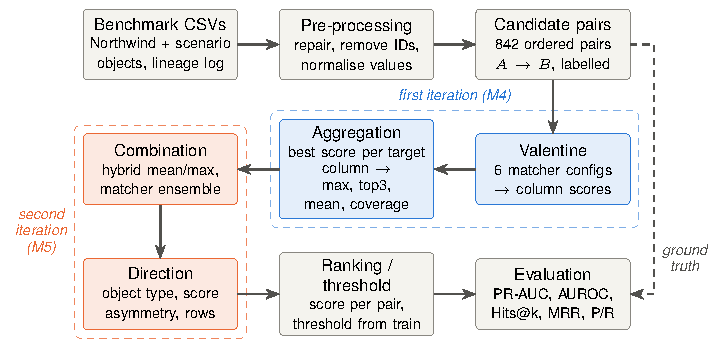
\includegraphics[width=0.9\linewidth]{pipeline.pdf}
\caption{Our pipeline. Blue: first iteration (Milestone 4). Orange: second iteration (Milestone 5).}
\label{fig:pipeline}
\end{figure}

\paragraph{Matchers.} We use six settings with default parameters: COMA with and without values, Cupid and
Similarity Flooding (names), and Jaccard and distribution-based (values).

\paragraph{From column scores to one table score.} For each column $b$ of the target table we take its best score
$s_b$ over all source columns. Then we combine these scores into one number in four ways: \texttt{max} (the best
column), \texttt{top3} (mean of the three best), \texttt{mean} (mean over all target columns) and \texttt{coverage}
(share of target columns with $s_b \geq 0.5$).

\paragraph{Second iteration: combining.} We try (1) a mix of \texttt{mean} and \texttt{max},
$w \cdot \texttt{mean} + (1-w) \cdot \texttt{max}$, (2) the average of several matchers, and (3) \emph{stacking}: a
logistic regression that uses all 24 scores (6 matchers $\times$ 4 aggregations) of a pair as input. We train it on
the train split only and choose its regularisation with cross-validation.

\paragraph{Second iteration: direction.} The matching score is almost the same in both directions, so it cannot
tell which table came first. We test three simple rules: (1) the score of $A \rightarrow B$ against the score of
$B \rightarrow A$, (2) the table with more rows comes first, and (3) the object type order: original table $<$ view
$<$ table $<$ temporary table $<$ final table. We also test a weaker version of (3) that only says that original
tables come first. If the rule says that a pair has the wrong direction, we set its score to 0.

% ---------------------------------------------------------------------------------
\section{Experimental setup}\label{sec:setup}

\paragraph{Train and held-out data.} Valentine itself is not trained. Every choice (which matcher, weights,
threshold) is made on the \emph{train} split. We report results on \emph{test} and \emph{multi} together (19 of the
30 links), which we call held-out.

\paragraph{Metrics.} Only 3.6\,\% of the pairs are real links, so accuracy is not useful. We treat the scores as a
ranking and use PR-AUC and AUROC over all pairs. For every derived table we also rank all possible source tables and
report Hits@1, Hits@3 and the mean reciprocal rank (MRR). In addition we report precision and recall at the best
threshold of the train split.

\paragraph{Baselines.} (1) Random scores, (2) the similarity of the table names, and (3) \emph{value containment}:
the share of each target column's values that we find in one source column, averaged over the target columns. This
is a simple value matcher that we wrote ourselves, without Valentine.

\paragraph{Comparison with the paper.} The GNN predicts row-level links in a knowledge graph and is tested against
4\,000 random negative examples. We predict table-level links. To get closer to their Hits@10, we also rank each
true link against 50 or 100 random negative pairs. These numbers are only a rough comparison.

\paragraph{Tools.} Python 3.13, Valentine 1.1, pandas, NetworkX and scikit-learn. Running all six matchers on all
842 pairs takes less than four minutes on a laptop. Notebooks \texttt{01}--\texttt{05} in our repository produce all
numbers in this report.

% ---------------------------------------------------------------------------------
\section{Results}\label{sec:results}

\subsection{First iteration}\label{sec:res-first}

\begin{table}[htbp]
\centering\small
\caption{Held-out results of the baselines and of the best aggregation of each matcher.}
\label{tab:first}
\begin{tabular}{llrrrrr}
\toprule
method & uses & PR-AUC & AUROC & Hits@1 & Hits@3 & MRR \\
\midrule
random & -- & 0.06 & 0.50 & 0.09 & 0.26 & 0.26 \\
table name similarity & names & 0.12 & 0.64 & 0.40 & 0.53 & 0.52 \\
value containment (ours) & values & 0.22 & 0.86 & 0.33 & 0.73 & 0.54 \\
\midrule
Similarity Flooding + top3 & names & 0.07 & 0.64 & 0.13 & 0.47 & 0.36 \\
Cupid + mean & names & 0.17 & 0.84 & 0.27 & 0.67 & 0.48 \\
COMA (names) + mean & names & 0.18 & 0.78 & 0.20 & 0.47 & 0.45 \\
Distribution-based + mean & values & 0.19 & 0.79 & 0.33 & 0.53 & 0.52 \\
COMA (names + values) + mean & both & 0.20 & 0.85 & 0.33 & 0.60 & 0.55 \\
Jaccard + mean (chosen on train) & values & 0.21 & 0.86 & 0.40 & 0.73 & 0.59 \\
\bottomrule
\end{tabular}
\end{table}

\begin{figure}[htbp]
\centering
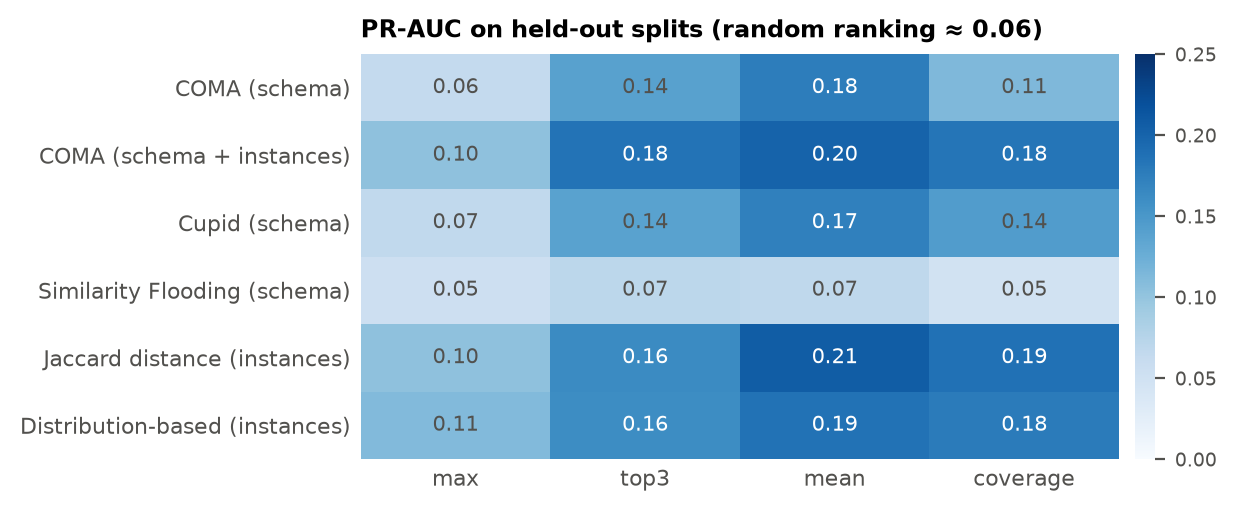
\includegraphics[width=0.7\linewidth]{exp_01_prauc_grid.png}
\caption{Held-out PR-AUC for every matcher and aggregation.}
\label{fig:grid}
\end{figure}

Table~\ref{tab:first} and Figure~\ref{fig:grid} show the results of the first iteration. The matchers that use
values work best (Jaccard, COMA with values, distribution-based). The best matcher that only uses names, COMA,
reaches 0.18, and Similarity Flooding is almost as bad as random. This is what we expected from the data analysis.
For every matcher, \texttt{mean} is the best way to combine the column scores, because a derived table usually takes
most of its columns from its source, while \texttt{max} is often fooled by a single shared key column.

The setting chosen on train, Jaccard with \texttt{mean}, is also the best one on the held-out data. It is about 3.5
times better than random, but our own simple value containment baseline is just as good (0.22 vs.\ 0.21). This
makes sense, because the Jaccard matcher measures almost the same thing.

\paragraph{Errors.} At the best train threshold, precision is 0.27 and recall is 0.32. However, all wrong
predictions are pairs from the right lineage chain: either the direction is wrong (\texttt{FinalAtRiskLog}
$\rightarrow$ \texttt{tempAtRisk}) or the link skips a step (\texttt{Orders} $\rightarrow$ \texttt{OrderSummary}).
No unrelated pair is predicted. The direction is correct for only 18 of the 30 links. The links with the lowest
scores are (1) bridged links, (2) source tables that give only one column to a join view, for example
\texttt{Customers} and \texttt{Shippers} $\rightarrow$ \texttt{vwOrderFulfillment}, and (3) links where the columns
are computed, so neither names nor values match.

\subsection{Second iteration}\label{sec:res-second}

\begin{table}[htbp]
\centering\small
\caption{Second iteration, held-out results. Everything is fitted on train.}
\label{tab:second}
\begin{tabular}{lrrrrr}
\toprule
system & PR-AUC & AUROC & Hits@1 & Hits@3 & MRR \\
\midrule
first iteration (Jaccard + mean) & 0.21 & 0.86 & 0.40 & 0.73 & 0.59 \\
mix of mean and max ($w = 0.2$) & 0.20 & 0.84 & 0.40 & 0.73 & 0.60 \\
average of 6 matchers & 0.21 & 0.85 & 0.40 & 0.87 & 0.64 \\
stacking (logistic regression) & 0.25 & 0.86 & 0.40 & 0.93 & 0.65 \\
stacking + original tables first & 0.26 & 0.87 & 0.40 & 0.93 & 0.65 \\
\textbf{stacking + object type order (final)} & \textbf{0.36} & \textbf{0.92} & \textbf{0.60} & \textbf{0.93} & \textbf{0.76} \\
\bottomrule
\end{tabular}
\end{table}

\paragraph{Table names.} We ran all matchers again with table names without prefix and with meaningless names
(\texttt{aaa}, \texttt{bbb}). COMA, Cupid and Jaccard give exactly the same scores, and Similarity Flooding and the
distribution-based matcher change by less than 0.01 PR-AUC. So the table names in the benchmark do not make the task
easier for Valentine.

\paragraph{Mixing mean and max.} This does not help. Only pure \texttt{max} is bad; with any amount of
\texttt{mean} the result is the same as \texttt{mean} alone (0.20 vs.\ 0.21). When \texttt{max} moves single-column
join sources up, it also moves up all pairs that share a key column.

\paragraph{Combining matchers.} Averaging matchers changes little (Table~\ref{tab:second}), because the matchers
make the same mistakes. Stacking works better: PR-AUC goes from 0.21 to 0.25, Hits@3 from 0.73 to 0.93 and MRR from
0.59 to 0.65. The model gives high weights to Cupid and to the value-based scores, and negative weights to the
name-based \texttt{max} scores of COMA and Similarity Flooding. Since train has only 11 positive pairs, this result
should be seen as a first indication.

\begin{table}[htbp]
\centering\small
\caption{How often each rule finds the right direction for the 30 true links.}
\label{tab:direction}
\begin{tabular}{lrrr}
\toprule
rule & correct & no decision & wrong \\
\midrule
score $A \rightarrow B$ vs.\ $B \rightarrow A$ & 18 & 6 & 6 \\
more rows first & 9 & 14 & 7 \\
original tables first & 14 & 16 & 0 \\
original tables first, then score, then rows & 22 & 5 & 3 \\
object type order & 29 & 1 & 0 \\
\bottomrule
\end{tabular}
\end{table}

\paragraph{Direction.} Table~\ref{tab:direction} shows that the object type order finds the right direction for
29 of the 30 links, while the score alone finds 18 and the number of rows only 9 (join views have more rows than
their small source tables). When we use the object type order to remove reverse pairs, PR-AUC rises to 0.36, AUROC
to 0.92 and MRR to 0.76. The weaker rule (only ``original tables first'') never makes a mistake, but it only decides
14 links and hardly changes the ranking. We have to be careful here: the object type order comes from the naming
convention of the benchmark (\texttt{vw\_}, \texttt{Table\_}, \texttt{\#\#Temp}, \texttt{Final\_}).

\begin{figure}[htbp]
\centering
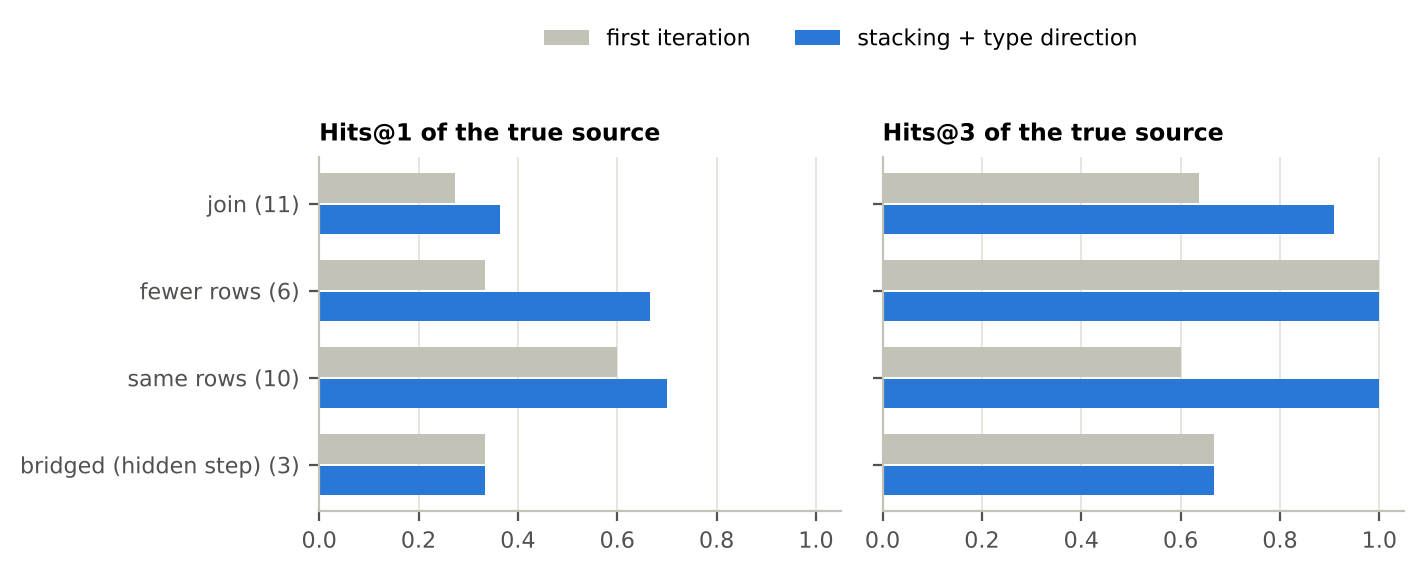
\includegraphics[width=0.82\linewidth]{it2_03_scenarios.png}
\caption{Hits@1 and Hits@3 of the true source by type of lineage (11 join, 6 fewer rows, 10 same rows and 3 bridged
links).}
\label{fig:scenarios}
\end{figure}

\paragraph{Types of lineage.} Figure~\ref{fig:scenarios} splits the results by type of lineage. Joins are the
hardest case in the first iteration (Hits@1 0.27), because small source tables like \texttt{Shippers} give only one
column to the view. With the final system, the true source is in the top 3 for 10 of the 11 join links. Links
where the target has fewer or the same rows as the source reach Hits@3 = 1.0. Bridged links are still hard; one of
them even drops from rank 1 to rank 10 with stacking.

\paragraph{Threshold.} With the best train threshold, the final system finds about half of the held-out links
(recall 0.53, before 0.32) with a slightly higher precision (0.34, before 0.27). But now only about two thirds of the
predicted pairs are in a true lineage chain, while in the first iteration all of them were. So the final system is
clearly better as a ranking, but the threshold still needs work.

\subsection{Comparison with the paper}

\begin{table}[htbp]
\centering\small
\caption{Rough comparison only. The GNN predicts row-level links, we predict table-level links. Paper values are
averages over the tasks in Table~3 of~\cite{dutkiewicz2026rddl}.}
\label{tab:paper}
\begin{tabular}{lrrrr}
\toprule
system & precision & recall & AUC (PR) & Hits@10 \\
\midrule
GNN, RDDL ontology (9 tasks) & 0.91 & 0.90 & 0.92 & 0.68 \\
GNN, RDDL ontology (3 join tasks) & 0.85 & 0.86 & 0.86 & 0.62 \\
Valentine, first iteration & 0.27 & 0.32 & 0.21 & 0.74 / 0.53 \\
Valentine, final system & 0.34 & 0.53 & 0.36 & 0.88 / 0.75 \\
\bottomrule
\multicolumn{5}{l}{\footnotesize Valentine Hits@10 against 50 / 100 random negative pairs.}
\end{tabular}
\end{table}

The two evaluations are different in several ways: row-level vs.\ table-level links, 4\,000 negatives vs.\ all
tables of a split, the full benchmark vs.\ three CSV exports, and a trained vs.\ an untrained model. So
Table~\ref{tab:paper} only gives a rough idea. On Hits@10 against 50 negatives, Valentine is in the same range as
the GNN (0.88 for our final system, 0.57--0.74 for the RDDL tasks), but precision and recall are much lower than
the GNN's values of about 0.9. On the other hand, Valentine needs no training (the GNN uses about 5 million
training samples per graph), works directly on the tables, runs in a few minutes, can be used on a new database
right away and shows which columns were matched (for example \texttt{CompanyName} $\leftrightarrow$
\texttt{CustomerName}). Its weak points are the direction of a link, finding the exact link inside a chain, and
computed columns.

% ---------------------------------------------------------------------------------
\section{Discussion and limitations}\label{sec:discussion}

Our own simple value matcher is as good as Valentine's best single matcher. So on this benchmark the main benefit
of Valentine is not a better signal, but a ready-to-use tool that needs no training, explains its results and offers
several matchers that can be combined. Because its top results are almost always in the right lineage chain,
Valentine could be used to suggest candidate links that a person or a stronger model then checks.

The main limitations of our work are:
\begin{itemize}
  \item \textbf{Direction rule.} The object type order follows the naming convention of the benchmark. In a real
        database we would need other information, such as the creation time of a table. With the weaker rule the
        improvement disappears.
  \item \textbf{Small training set.} Stacking is trained on only 11 positive pairs, so the weights may not work as
        well on other databases.
  \item \textbf{Missing evidence.} Bridged links and computed columns (41\,\% of derived columns) cannot be found
        with names or values.
  \item \textbf{Data.} We only use three CSV exports, not the full benchmark, and there are no union scenarios in
        them. With 30 links, single links have a big effect on the metrics.
  \item \textbf{Level.} We predict links between tables, not between rows like the GNN.
\end{itemize}

% ---------------------------------------------------------------------------------
\section{Conclusions}\label{sec:conclusions}

We tested whether Valentine, a schema matching tool that needs no training, can find missing table-level lineage
links. On the Northwind lineage benchmark, the value-based matchers rank true links much higher than random
(PR-AUC 0.21 vs.\ 0.06), and their top results are in the right lineage chain. Combining the matchers with a
logistic regression and adding a direction rule raises PR-AUC to 0.36 and MRR to 0.76. Valentine does not reach the
precision of the GNN, but it is fast, simple to use and easy to explain. The table names do not affect its scores.
The main problems are the direction of a link, join sources that give only one column, and links through deleted
temporary tables.

In future work we would like to find the direction from information that a real database has (for example creation
time), test on the full benchmark, try language-model matchers such as Magneto~\cite{liu2025magneto}, and write the
predicted links as \texttt{tableDerivedFrom} triples into the RDDL knowledge graph.

\bibliographystyle{plainnat}
\bibliography{refs}

\end{document}
